\documentclass[a4paper]{article}

\usepackage{graphicx}
\usepackage{float}                                              % Required to use [H] in figures.
\usepackage[colorlinks=true, urlcolor=blue]{hyperref}           % For hyperlinks
\usepackage[margin=1.0cm]{geometry}                     % Set the left margin
\usepackage{tabularx}
\graphicspath{{png}}                                            % Set the default path for images.
\DeclareGraphicsExtensions{.png}                                % Only use image files with .png extension.
\linespread{1.30}                                               % Set line-height.

\hbadness=99999  % or any number >=10000
\vbadness=99999  % or any number >=10000

\begin{document}

    Eric Findlay

    \verb|e.findlay@protonmail.ch|

    \verb|https://github.com/currency-engineering|

    In the early 1970s, the physicist Henri Rathgeber applied his training to the problem
    of macro-economic control, and in particular unemployment. His solutions were too ahead of their
    time to gain any attention. At the time he only had access to Australian unemployment and
    inflation data. I have re-articulated his reasoning, extended it and re-tested his theories with
    the large body of economic data now available. The result is a solution to a problem considered
    by David Hume in the 1770s, namely if currency is simply a unit of purchasing power one expects
    a doubling of money to have to real effects. On the contrary Hume observed that silver and gold
    flowing in from the Americas had the effect in increasing economic activity. Hume implicitly
    assumed that currency, something we can now think of as a digital system, was important, together
    with the human interaction and decision making through market processes. Now if currency is
    indeed important we must ask what techniques could be best used to attack the problem.
    Rathgeber's fundamental insight was this kind of problem required an engineering approach, and
    in particular the use of control system engineering. The application of these methods results
    relatively straightforwardly in a good understanding of currency and economic systems.

    \begin{figure}[H]
    \centering
    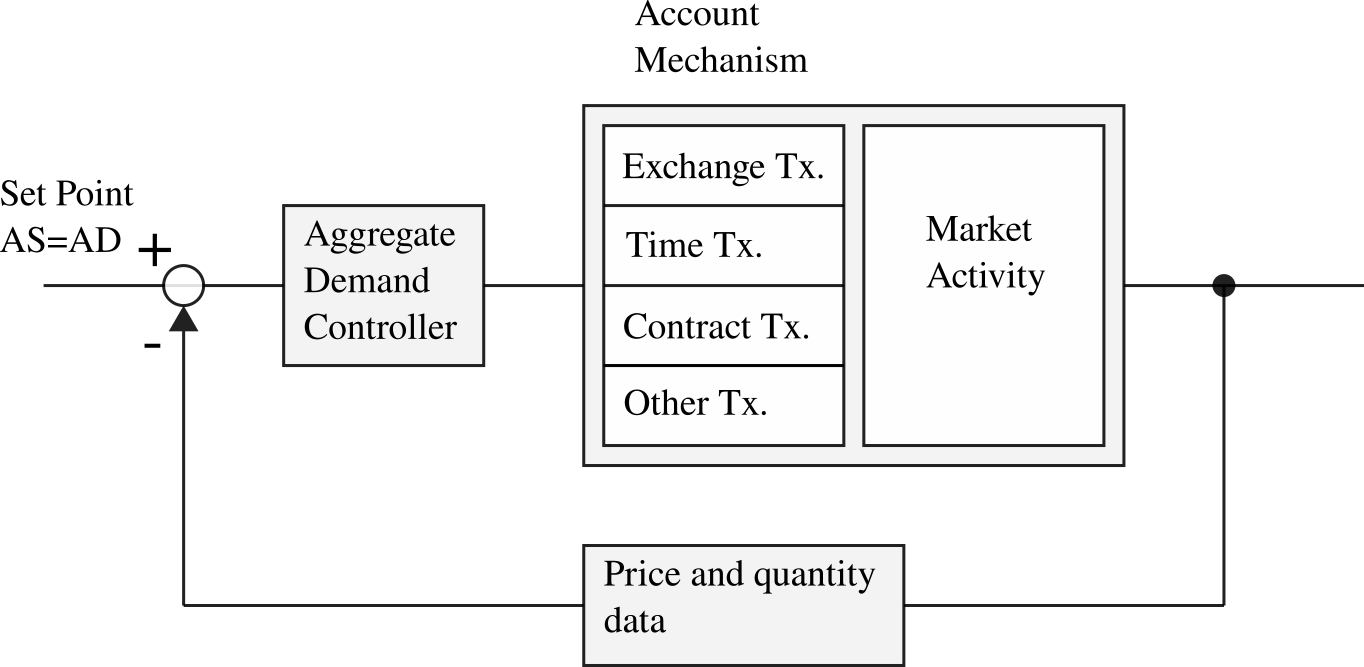
\includegraphics[scale=0.50]{economic_feedback_schema}
    \end{figure}

    We identify three constraints or instabilities. Handling errors is an important requirement
    in all control systems. If there is an error rate that reduces economic agreements to actual
    transactions, we can determine a fundamental constraint on the markets equilibriation process as
    shown. Inflating the currency is an error correcting mechanism, which explains Hume's question
    of why increasing the supply of money increases economic activity. There is a destabilizing
    interaction between exchange transactions and lending transactions. Irving Fisher in 1908 showed
    that the interest rates written into contracts for lending must be adjusted to changes in the
    inflation rate. This results in a positive feedback instability where increases in the inflation
    rate force increasing real costs of production. Contract transactions are distinct from lending
    transactions and involve a payment for a change in contract status or ownership. A positive
    feedback instability occurs when the price of contracts changes over time and people enter the
    market to speculate on these changes. 

    The control solution is to separate out the different kinds of transactions types into an
    abstraction layer that sits over accounts. Destabilizing interactions can the be prevented by
    decoupling the transaction types by using the following mechanisms:

    The error constraint is an unavoidable condition that can only be compensated for with
    sufficient inflation. The instability inducing interaction between exchange transactions and
    time transactions can be decoupled by using a unit of account of constant purchasing power in
    which to write contracts. This allows the inflation rate to be controlled without inducing
    instabilities. The instability in contract transactions can be eliminated by removing contract
    transactions entirely (time transactions are available for productive investment). This can be
    done by ensuring that repayments for lending must be directly from borrower to the original
    lender. Also be removing contract transaction functionality, we prevent bank accounts, allowing
    a monetary authority or algorithm to directly and precisely control aggregate demand by
    adjusting the purchasing power of all accounts in exact proportionality.

    All currency designs up to date prevent constrain economic participants from driving markets
    to equilibrium, resulting in an unpredictable economy with sustained unemployment and poverty.
    Because digital currencies allow for the possibility of an abstraction layer over accounts,
    digital currencies are a means of implementing a currency design that is likely to solve
    fundamental economic problems. This abstraction layer is in general hidden from the account
    owner and accounts appear very much like accounts in any other digital currency. 

    My hope is to build a open-source digital currency in Substrate to test as a prototype, and to
    communicate the design requirements of working digital currencies to others.

\end{document}

